\documentclass[
	%parspace, % Add vertical space between paragraphs
	%noindent, % No indentation of first lines in each paragraph
	%nohyp, % No hyphenation of words
	%twoside, % Double sided format
	%draft, % Quicker draft compilation without rendering images
	%final, % Set final to hide todos
]{elteikthesis}[2023/04/10]

% The minted package is also supported for source highlighting
% See minted-intregration.tex for example
%\usepackage[newfloat]{minted}

% Document's metadata
\title{Traffic Control and Infrastructure Organization Using Reinforcement Learning} % title
\date{2023} % year of defense

% Author's metadata
\author{Dániel Kuknyó}
\degree{IT for Autonomous Systems MsC.}

% Superivsor(s)' metadata
\supervisor{Dr. András Lőrincz} % internal supervisor's name
\affiliation{Head Senior Researcher} % internal supervisor's affiliation
%\extsupervisor{Jane Doe} % external supervisor's name
%\extaffiliation{Senior Developer} % external supervisor's affiliation

% University's metadata
\university{Eötvös Loránd University} % university's name
\faculty{Faculty of Informatics} % faculty's name
\department{Dept. of Software Technology and Methodology} % department's name
\city{Budapest} % city
\logo{elte_cimer_szines} % logo

% Add bibliography file
\addbibresource{elteikthesis.bib}
\bibliography{elteikthesis}

% The document
\begin{document}

% Set document language
%\documentlang{hungarian}
\documentlang{english}

% List of todos (not in the final document)
%\listoftodos[\todolabel]

% Title page (mandatory)
\maketitle
% Topic declaration page (mandatory) - can also be attached instead
%\includepdf{topicdeclaration.pdf}

\tableofcontents{}\newpage{}

\chapter{Introduction}

\section{Motivation}

In recent years the traffic of cities became a rising topic with more
and more city governments realizing that a motor focused city design
is unsustainable. Cities all around Western Europe have started designing
their cities around humans and public transit, and not around cars.
E.g. Paris is planning to be a 15-minute city, Barcelona is incorporating
the superblock design, Finland is creating non-intersecting paths
between the common intersections and the Dutch are using intelligent
traffic light systems to manipulate traffic flow in order to optimize
it for both cars and pedestrians. 

If one takes a look at how the Dutch infrastructure is designed, they
will see that despite having less car lanes and overall less space
for cars, the traffic flows more dynamically. This is thanks to the
intelligent design of intersections, traffic lights and infrastructure.
The methodology of this has been known ever since the 1970s, but the
auto industry has been fighting against it ever since in order to
gain more market. In Northern America one can observe what happens
if a city is designed with cars in mind, requiring everyone to own
a vehicle in order to participate in society. This results in worse
accessibility to the public for the disabled, incapable, elderly and
young people as well with less sense of community, relationships.
The approach to creating walkable, human-centered and intelligent
infrastructure that is optimal for both pedestrians and cars is laid
out in detail in the literature such as Strong Towns, a non profit
urban planning organization.

The aim for this research is to able to model a system of roads or
city, and being able to pinpoint mistakes made by development engineers,
with the goal in mind to make the city more humanly livable, liquidate
urban highways and make traffic infrastructure more efficient for
the benefit of both humans and motorists. This is a key aspect in
designing the future's cities and the way to have a more sustainable
living ecosystem.

\section{Goals and outline}

The project will focus on building an environment that models traffic
flow in a graph-based structure, then to train a reinforcement learning
model to find the optimal configuration of the roads in order to transport
the most cars in the most effective way possible. This is an expert
area where the urban design principles play a key role: one can easily
observe that the most effective way to transport as many cars as possible
is if all roads are 8-lane highways. However it's also easy to see
that it's miserable to live in a city where there are no quiet, auto-low
streets and only 8-lane highways. This might be the best configuration
for cars, but it would make the life of people living in the city
absolutely horrible. 

The reinforcement learning agent's goal is to learn how to create
a city where it's nice to live for a human and fast to drive for a
vehicle through building and destroying infrastructure. The goal of
the rewarding system of the reinforcement learning environment is
to express these ideas: building cost, traffic light/roundabout trade
offs, how humans would feel living next to the road. The agent will
have to decide where to build, destruct, or make roads 1-way to make
the city's transportation flow dynamic but also make it livable for
humans. The rewarding scheme is expected to reflect the principles
laid down by Strong Towns and other urban planning organizations significant
in the field like Happy Cities: Transforming Our Lives through urban
design. The main metrics that are taken into account during the research
are:
\begin{enumerate}
\item Time taken to arrive to the goal junction
\item Cost of infrastructure
\item Livability by humans (number of lanes, connection density)
\end{enumerate}

\section{Research hypotheses}

If the research is successful, the following hypotheses can be verified
or nullified: 
\begin{enumerate}
\item Can traffic flow and driver behavior be modeled inside a reinforcement
learning environment accurately enough for it to be representative
of the real world?
\item Can predefined road configurations be optimized for traffic flow,
human livability and cost efficiency at the same time?
\item Is there a single neural network architecture that can achieve the
optimization in every configuration or there is a need for a more
complex neural network as the complexity of the graph increases? 
\end{enumerate}
\newpage{}

\chapter{Research Background}

\section{City Design}

\subsection{A brief history of the modern day street}

The shape and fabric of cities is the result of hundreds or thousands
of years of development, transformation and reshaping. Many geographical
and historical events play a role in determining how a city's transportation
infrastructure is designed. The industrial revolutions have been the
key driving events of change in most countries as they have led to
the transformation of the pedestrian centered traffic. The most significant
factor in city design has always been some idea of happiness or philosophy.
E.g. the \emph{agora} in ancient Athens, which was essentially a main
square. However the philosophy of good life was built into it as it
can be observed through monuments, temples, the most important buildings
and law courts that have been surrounding it. And this practice of
building and designing architecture hasn't changed ever since \cite{jette2013book}.
Even today, when a new skyscraper is built, it will reflect the architect's,
CEO's or other executive members' ideas of happiness or greatness.
They will look at it, and decide if they like it: is it good to go
for building or not. But what has changed since ancient Greece? What
was the key motive that made us design cities focused around cars? 

Philosophy has always been a pendulum oscillating between sky and
earth - God and human. In the Middle ages, the focus was God. Then
following it in the Renaissance, the human became the focus of inspiration.
After that came the Baroque, again with God as the main motivator.
After the Enlightenment and the birth of the modern day citizen, the
first style trend was Rococo, focused around humans. Around this time
has religion lost its status as the main, unified cultural narrative
as it can be observed in the works of Nietzsche and Derrida \cite{williams2012tragedy}.
The last attempt at constituting God as the center of philosophy was
in the style trend of Romantics. However as the modern era citizen
of the Enlightenment wasn't religious anymore, the style attempted
to find God in the human (übermensch - Nietzsche). This is expressed
in various other fields, not just architecture or city design: art,
poetry, statuary, astronomy and even mathematics. The loss of focus
around God and religion in modern society can also be seen as a contributing
factor to the shift in urban planning towards car centric cities.
With the decline of traditional religious institutions and values,
there has been a shift towards individualism and consumerism in Western
societies. The car, as a symbol of personal freedom and mobility,
has become a powerful cultural icon that reflects these values. In
contrast, traditional urban planning, with its emphasis on public
transportation, walkability, and community spaces, was often based
on religious values and ideas about communal living. The decline of
religious institutions and values also led to a decline in the importance
of shared public spaces, such as parks, town squares, and community
centers. These spaces, which were often designed to promote social
cohesion and a sense of community, were gradually replaced by private
spaces such as shopping malls and suburban subdivisions, which were
designed around individual consumer preferences and the use of private
cars.

Around a hundred years ago in the 1920s cars have begun to appear
in the cities in greater and greater numbers. At first it was a new
and expensive technology, hence it was mostly the wealthy class that
owned them. At this point in time traffic rules were essentially nonexistent,
so drivers could drive however they pleased. This quickly led to a
large number of traffic related incidents. This was a massively bad
PR for the auto industry, so they started influencing city design
using their political and economical capital \cite{marshall1996injuries}.
In school the children started to receive education about having to
look both ways before crossing the road \cite{norton2011fighting},
because they are the ones that don't belong on the road and not the
other way around. Peter Norton argues \cite{norton2007street} that
the crucial moment in the shift towards car centric urban design occurred
in 1923, when Cincinnati residents were asked to vote on a proposal
to impose a 25 mph speed limit on drivers. This measure would have
made it difficult for car dealerships to sell cars, potentially leading
to a decline in revenue, business, and political influence. As a result,
representatives of the automobile industry launched a concerted effort
to defeat the measure, using tactics such as billboards, fliers, and
even paying people to vote against it. Ultimately, the auto industry
emerged victorious, gaining significant political and economic influence
over the subsequent years.

\subsection{The current state of city design}

Ever since, car dependent infrastructure and lifestyle is thriving
in the USA. Owning a private vehicle has become a minimum requirement
to take part in society as the sprawl has led to a run down public
transit and railway infrastructure. As of the current state, the automobile
is dominating the transport in the USA and hence becoming one of the
most important determinants of the American lifestyle \cite{pucher1996united}.
This can be attributed to the way cities and residential buildings
are designed. A typical American city has overwhelmingly two types
of residential buildings: skyscrapers and high rise buildings downtown
and low density suburban expansion around it. What's missing is a
trade off between the two: mid density, mixed use housing that can
at the same time house a sufficient amount of people in a relatively
small area, but at the same time is relatively cheap to build in comparison
with skyscrapers. This mid density residential housing planning would
be the key guarantee to design walkable neighborhoods in the United
States, however it's missing. Of course, there are some areas where
this type of architecture can be found but this is not the norm, it's
the exception. This is referred to as the missing middle problem \cite{parolek2020missing}.
This is partly because zoning laws in the USA don't make it possible
to build this type of building. The remaining buildings are so spaced
out because according US regulations there's a parking minimum for
every building built. Parking minimums are requirements set by local
governments or zoning codes that specify the minimum number of parking
spaces that must be provided for a particular type of development.
For example, a zoning code may require that a new apartment building
must provide one parking space for every unit, or that a new office
building must provide one parking space for every two employees.

From the way the cities are built comes car dependency as a consequence.
However this has also led to public transit being underdeveloped:
the housing density in the suburbs doesn't reach the threshold to
make it worth making it being part of a bus or train route. No matter
where the city puts the bus stop, the time taken to get there on foot
in the area is too much for people not living near it. Putting bus
stops overall would require too much public transit infrastructure
that would have to be subsidized from taxpayer money and would result
in near empty buses. The optimal scenario is when a transit route
can reach just enough people so that the maintenance and operation
can be financed from ticket fares and minimal amount of subsidies.
This is called the critical density. If there is a critical density
reached a single transit stop can serve enough people, which will
make it worth in fare revenue. It's also rare to find dedicated bus
and cycling lanes in the USA. 

Buses are generally stuck in traffic with the cars in rush hour, which
makes it even less inviting for passengers. It's worthwhile to note
here that adding lanes to an already existing road does not solve
traffic, so it's not a solution to just make roads wide enough so
that buses don't have to wait in line together with motor vehicles.
As an example consider the recent expansion to the I-10 highway south
of Houston known as the Katy Freeway. Together with a recent expansion,
it's now at 26 lanes at its widest part at the time of writing but
traffic jams are a regular occurrence. Adding lanes also reduces the
safety of the road, as found by \cite{milton1998relationship} who
were analyzing the relationship between the road geometry and safety,
and also \cite{abdel2000modeling}, who found a positive correlation
in the numbers of crashes and the number of lanes in urban highway
road intersections. Dedicated bike lanes are also missing from the
infrastructure: the most common cycling lanes one can find are painted
bicycle gutters without any separation from high speed motor traffic
that makes it very dangerous to ride a bicycle. This results in even
more inequality in society. 

Apart from the reasons mentioned before, car dependency has another
different aspect, $CO_{2}$ emissions. A study has found that despite
being 5\% of the total population, the United States is responsible
for 45\% of all transportation $CO_{2}$ exhalation \cite{decicco2006global}.
A different work in the field suggests that the most transport emissions
could be reduced by converting low density housing to mid density
\cite{gately2015cities}. Even more than converting mid density to
high density.

\subsection{The stroad}

The stroad is a term created by a non-profit urban planning organization
called Strong Towns that has been referred to and processed by several
relevant pieces of literature like the book Confessions of a Recovering
Engineer - Transportation for a Strong Town \cite{marohn2021confessions}.
The idea of the stroad lays down the guidelines which have to be reflected
during the training phase of the agent as it highlights some key aspects
of city design. To be able to understand the the stroad as a concept,
it's necessary to first grasp the functions and purpose of a road
and a street.

\subsubsection*{The road}

A road is a means of fast transportation between different destinations,
designed with wide and forgiving features to accommodate high-speed
travel. In order to keep vehicles at a maximum speed for as long as
possible, exits on the road are spaced far apart to reduce the number
of intersections. This also helps to prevent drivers from needing
to brake frequently, which can increase the risk of accidents. Turning
lanes are often included on many roads to allow drivers to slow down
before taking an exit, reducing the potential for danger. Adjacent
to the road is a clear zone that is kept empty for emergency purposes,
such as allowing vehicles to stop or for emergency vehicles to bypass
a line of traffic. The font size on road signs is large, making them
easy to read from a distance. The M3 highway in Hungary is an example
of a road that has been optimized for safety and fast travel. As important
pieces of infrastructure, roads play a crucial role in transportation
and safety.

\subsubsection*{The street}

The street is a densely populated environment that is primarily intended
for human use. It serves as a complex space where city life occurs,
and is therefore typically lively with people. The street is designed
for low-speed travel, as it is considered a destination rather than
a thoroughfare. High-speed traffic is incompatible with human activity,
as it introduces an added element of danger to commuting. Buildings
are often constructed directly adjacent to the sidewalk, making them
easily accessible to pedestrians. The street itself can be likened
to an outdoor room, where everything is scaled down to the size of
human beings. It is designed to be welcoming and inviting to those
who wish to walk, socialize, window shop, or simply breathe in some
fresh air. Many shops, restaurants, cafes, and services have entrances
and exits directly onto the street. Living near a well-designed street
can also increase the value of a property. The difference in real
estate prices between a flat near Váci Street versus one near the
M3 highway is a testament to how much society values human-centered
design in urban planning. Streets play a vital role in tourism, livability,
and overall quality of life within a city.

\subsubsection*{The stroad}

The stroad is a name that's the result of the combination of the words
street and road. It describes an urban motorway that is neither a
street nor a road, despite trying to be both of them. The stroad is
a street that's designed like a road, and doing so it fails to bring
forth the advantages of either of them, but is struggling with the
disadvantages of both of them. First the stroad is analyzed from the
viewpoint of a road.

On the stroad there are many entrances and exits to businesses and
services, like one would find on a street. However there are multiple
lanes of high-speed motor traffic in both directions. This is an added
factor of danger, as there are typically no dedicated turning lanes,
so drivers have to pay constant attention if the car in front of them
is taking a turn. Because of the high speeds involved this means that
drivers have to come to a quick halt. It's not rare that stroads allow
the 70 km/h speed limit, which drivers often surpass, because the
stroad is straight and wide. The geometry of the street allows the
drivers to reach higher speeds while still feeling safe, however this
is a fake sense of safety, as there are more points of conflict than
on a dedicated highway \cite{marohn2012thoughts}. Roads can keep
vehicles on high speeds because there are few exits. Traffic jams
are also a common occurrence. Because of the large distances involved,
walking feels very uncomfortable in this kind of environment. People
don't feel safe walking next to high-speed motor traffic. It's also
common that one can find large parking lots, which are also not inviting
for the human as there's nothing to see or do there. It's also difficult
to cross the stroad unless using a dedicated crosswalk and treading
very carefully not to be involved in an accident. This is clearly
a place for cars so it's not surprising that pretty much everyone
drives here. 

Next the stroad is evaluated from the point of view of the road. On
the stroad the lanes are wide and there are a lot of them. Traffic
flow is more chaotic than on the road because there are a lot of exits,
hence cars change lanes more often, easily giving the change to dynomen
situations: when there's no imminent danger, but the conditions can
turn dangerous at any moment. This also reduces the speed of traffic
flow. Cars changing lanes are the leading cause of the caterpillar
or butterfly effect. Traffic volumes are also high as often there
are no viable alternatives to driving: bus and cycle lanes are nonexistent.
This kind of car dependent infrastructure creates distances that only
cars can bridge, but not everyone owns a car in society. This city
design inherently widens the gap between the different layers of society.

Stroads are also very expensive, as they are built to a highway standard
despite the fact that they can't be used as efficiently: with high
speeds, while maintaining a strict level of safety as in the degree
of slope, sharpness of turns and several other design decisions that
have dedicated highway engineering and maintaining offices in almost
any country. The density of intersections requires the city to install
traffic lights, as they are the only type of intersection that can
be operated with a related safety for a road of this scale. Traffic
lights in the US can cost up to \$750.000 for an intersection. Roundabouts
and right hand priority intersection are not viable options here because
of the high speeds involved. Drivers need to see if they have to slow
down ahead of time.

The majority of crashes within the United States happen on stroads.
People walking and cycling are especially in danger as there's no
infrastructure that separates them from high-speed motor traffic.
The wide and open design of the stroad encourages drivers to drive
fast and not pay attention to their surroundings \cite{bates2015mixed}.
As an example, during the coronavirus lockdowns in the beginning of
2020, people weren't traveling as much, hence miles traveled by drivers
decreased. Despite 355 million less miles driven fatal car crashes
per mile increased by up to 34\% \cite{motorvehicle2020}. This leads
to the conclusion that the reason stroads aren't killing
even more people is that they are usually so jammed up
that the drivers can't go fast enough to kill each other.

\section{Practical uses of the research}

Today a great percentage of a city's budget goes towards motor infrastructure
planning, building, expanding and maintenance. Many cities mostly
in North America keep building more new infrastructure that they can't
maintain causing a municipal insolvency. This is referred to as the
``growth Ponzi scheme'' named after the common investment fraud
strategy in the literature \cite{marohn2019strong}. It stems from
the fact that maintenance costs start to appear after decades of road
use, where it will be constant. It's easier to build roads than to
keep fixing all the roads that are in bad condition. It also has political
motivations as building a new road can serve as better PR than fixing
potholes. There's also a large rate of suburban sprawl in the US and
Canada, and lower density results in more infrastructure being built.
This is an urban design and an infrastructure design problem at the
same time. 

There are many solutions from the urban design side such as building
more dense housing or rerouting highway expansions to not destroy
historically dense neighborhoods that serve a good amount of people
with affordable housing and public transportation. It's also very
difficult to run transit lines through the suburbs because of the
low density. There's a lesser amount of people in the rational radius
of the bus stop where it's worth taking the bus rather than to walk
a long distance to a bus stop and then take the bus. For this reason
it's not common for US and Canadian suburbs to have widely accessible
transit lines going through them. 

Another principle is infrastructure design, which is the main focus
of this research. From an infrastructure design perspective careful
preparation and planning must precede the execution of building a
new piece of infrastructure or the expansion of an existing one. The
city must thoroughly consider where to spend its finite funds. This
is the aspect where this research can help in the decision making
process. The developed software and framework considers a new or existing
piece of infrastructure between junctions and optimizes it in terms
of traffic flow and human-centered perspectives. The goal of the deep
learning model is to find the optimal configuration which costs the
least amount of money while providing a maximal amount of capacity
expansion while still considering human factors in a traffic environment. 

There can be three very distinct use cases of the piece of software
that's being developed under the umbrella of the research:
\begin{enumerate}
\item Within-city: this use case comes down to optimizing an existing piece
of infrastructure. This use case has some restrictions: 
\begin{enumerate}
\item No new roads can be built between junctions as this would necessarily
mean destroying existing buildings. 
\item Only a limited number of lanes can be added to the existing roads. 
\item Junction types can be set freely. 
\end{enumerate}
\item Green field investment (Outside-city): in this problem the RL agent
is given junctions and it's free to set everything between them. The
hypothesis is that there are no existing roads, and the junctions
must be connected to each other in the best way possible:
\begin{enumerate}
\item Lanes and roads can be added freely.
\item Maximum number of lanes can be anything (within rational limits).
\item Junction types can be set freely. 
\end{enumerate}
\item Reparation mode (mixed): This is a mix of the previous two use cases.
The RL agent is given a current traffic system and the task is to
convert it to the best possible model while using a limited amount
of money and resources.
\begin{enumerate}
\item The junctions are given. 
\item Lanes and roads can be added, existing ones can be destroyed. 
\item Junction types can be set freely.
\end{enumerate}
\end{enumerate}
If the human factors weren't taken into consideration the problem
could be reduced into a maximization scheme where the target is to
find the fastest traffic flow. The solution to this problem seems
rather trivial: building 8-lane freeways between all the junctions. 
However a city like this can't be imagined within rational frames.
The true problem at hand is an optimization scheme for multiple variables
and ideas. The city budget and the experience of pedestrians must not be left
out of the equation. 

\section{Deep learning in Infrastructure organization}

\subsection{The spectrum of expert areas}

Predictions in new literature all point in one direction regarding
traffic control and artificial intelligence: AI will most likely become
the brain of infrastructure and traffic as well as many other expert
areas. With the rise of autonomous vehicles this possibility seems
closer than ever. There's a huge potential in operating, managing
and monitoring transportation. The infrastructure is going to be very
similar to that of the internet currently: a decentralized network
that is operated by mesh and local servers, data flow being sensor
readings coming to and going from the several vehicles on the road.
There are currently existing studies on the viability of smart networks
that infuse different kinds of sensors with road infrastructure \cite{hoult2009wireless}.
For public transportation the LOA and GOA frameworks lay down the
principles of creating an ethical AI-driven solution for trams and
trains respectively \cite{salo2021ai}. There are also works that
use traffic light governance systems enhanced by artificial intelligence
to aid faster traffic flow \cite{sukhadia2020optimization}. Reinforcement
learning has also been applied to control the cycle, phase and red/green
ratio of traffic light systems \cite{wei2021recent}. All of the studies
in the field can be placed on a spectrum that has the vehicle on one
end and the road infrastructure on the other. Some works develop systems
that enhance the vehicle, some are creating instruments for the road
that directly influence transportation safety or speed like traffic lights.
Others connect the road and vehicles together by infusing them with
intelligent sensors that add a level of safety to the traveling experience. 

\subsection{Infrastructure and building modeling}

Building information modeling (\emph{BIM}) is the collective name
for technologies and methods that aid the generation and modeling
the digital representations of places in order to have a better overview
of the building process. This introduces cost effectiveness, a level
of safety and better ways to understand environmental impact. Currently
transportation infrastructure is a keystone of its economy by providing
fast travel times for goods and orders, creating jobs thereby significantly
helping economical and social development. In recent years a great
need was shown for technologies that can increase the effectiveness
of building motor transportation infrastructure. There was a significant
development in the planning process for infrastructure. One of the
results of this development is BIM. BIMs are essentially computer
files that contain information on an object in order to help decision
makers and planners with design, building and overview. Different
kinds of dynamic data can also support BIMs like sensor measurements
and signals from the building systems. Advances in fields like computer
vision and artificial intelligence has given rise to a technological
revolution in building information modeling. There have been attempts
where building models were constructed using a combination of LIDAR
and photometric sensor data. BIM data itself is not an AI-driven process
but it can help aid AI-driven dynamic modeling by providing more accurate
information on buildings and infrastructure that can be part of a
data driven solution's environment model. BIM technology can be seen as both
a 3D model and the information that it represents. In this case the
model is more important as the representative of the information,
not just solely a model file \cite{kangari1990automation}.

BIM by itself is not a very new technology. In fact it has been around
since the 1980's. However combined with modern AI systems it can provide
planners and executors with more accurate information and in-depth
modeling. However in the recent years the interest in construction
tech has grown significantly. Construction tech is a larger collective
term for technologies and methods that aim at automating construction
and building processes. These can be mostly categorized into three
categories \cite{sacks2020building}: 
\begin{enumerate}
\item Planning: applications that aid the planning phase. These are mostly
software solutions for the designing and simulation of an environment.
Some companies are experimenting with AR (augmented reality) where
the planned building and the current state of construction are merged
into one simulated reality.
\item Sampling: these are software and hardware solutions that have the
goal of extracting information from the site. They are mostly sampling
and measurement devices that are now becoming far more advanced than
a simple laser ruler. LIDAR building scanners are an example.
The output of these devices often gets fed into the software that's
responsible for planning and modeling.
\item Construction: robotic hardware tools that actively build or destroy
infrastructure on the job site. Big leaps have been made in areas
such as transportation of material, applying paint and cleaning surfaces. 
\end{enumerate}
According to some estimates, venture capital investment in construction
technologies in the US reached as high as \$1 billion in 2018, which
translates to a fourfold increase from 2013 \cite{andersen2018state}.
This shows a large peak of interest in such technologies and gives
reason for further research in such fields of expertise.

\newpage{}

\chapter{Methodology}

\section{Constructing a city }

Everything starts with a city that the agent will have to learn and
optimize the structure of. At this point the city is best described
by a graph. Graphs are high-level descriptors of connections between
nodes. This gives an easy to use but highly customizable method to
define a city to train on. To define a city using the graph there
are two things that are needed to be defined: 
\begin{enumerate}
\item List of nodes of the graph with coordinates: $N_{1},N_{2},\ldots,N_{k}$.
\item List of connections between the nodes: $N_{i}\rightarrow N_{j},\ i\in1\dots k,\ j\in1\dots k$.
\end{enumerate}
These definitions together stored in a data file together are called
a \emph{construction protocol} from here on.

The developed software product provides an interface where the user
can make a graph, describing the intersections (nodes) and roads (edges)
of the city in question. The preferred interface to design a city is GeoGebra
\cite{geogebra2017geogebra}, where the graph can be exported into a construction 
protocol in order to work as an input for the model. Below is an example simple
city constructed:

\begin{figure}[H]
\begin{centering}
\includegraphics[width=10cm,height=10cm,keepaspectratio]{images/simple_graph}
\par\end{centering}
\caption{Graph-based representation of a city}

\end{figure}

The construction protocol is read into a graph, then the city is constructed
from it using an inner representation. As a starting configuration
every road is 2-way on the edges that have been set up in the graph.
The vehicle rate and distribution can be controlled before starting
the simulation. A constructed ``starting'' city according to the
previously shown graph looks like as follows:
\begin{center}
\begin{figure}[H]
\begin{centering}
\includegraphics[width=10cm,height=10cm,keepaspectratio]{images/simple}
\par\end{centering}
\centering{}\caption{The simulation running the same city. }
\end{figure}
\par\end{center}

So far this is a simple setup for demonstration. The dark rectangles
are vehicles on the road. The vehicles are passing from one entry
point to another, without necessarily choosing the shortest path,
or being evenly distributed among all the roads, just as one would
find in real life. The driver model is designed to incorporate intelligent
behavior like slowing down after the car in front is slowing down
or gradually speeding up with a comfortable rate of acceleration after
a light has turned green. 

The road configuration is to be examined with multiple metrics like how
many steps does it take for the roads to transport a given amount
of cars or how much the road infrastructure would cost. If the agent
is handed a road configuration it is expected to be able to find the
optimal one, with the least cost, least unnecessary roads and fastest
transportation for a given amount of cars. The cars are generated
using a predefined distribution and each traffic junction has a separate
entity of vehicle generator attached e.g. any graph node can be a 
spawn point for vehicles.

\section{Intelligent driver model}

The intelligent driver model (IDM) is a time-continuous car following
model for the simulation of urban traffic. It describes the behavior
of the drivers and the positions of vehicles. The model incorporates
the influence of one vehicle to another e.g. when some vehicle stops
the vehicle following it has to stop as well with a delay just like in 
real life. This property makes the model a good choice if the goal is to 
simulate real-world traffic as traffic jams, flash congestions and highway-like
behavior is built into the model. The following 6 parameters influence
how a driver behaves:
\begin{enumerate}
\item $v_{0}$: the desired velocity of the vehicle
\item $T$: safe following time
\item $a$: maximum acceleration
\item $b$: comfortable deceleration
\item $\delta$: acceleration exponent
\item $s_{0}$: minimum distance between vehicles
\end{enumerate}
The original model and the model that was used in this research was
invented by Treiber, Hennecke and Helbing \cite{treiber2000congested}.
For the sake of simplicity the same parameters are used all over the
simulation. The dynamics of the vehicle regarding acceleration and
deceleration counting in the leading vehicle are then described by
the following equations according to the authors:

\begin{equation}
\dot{x}_{\alpha}=\frac{\partial x_{\alpha}}{\partial t}=v_{\alpha}
\end{equation}

\begin{equation}
\dot{v}_{\alpha}=a^{(\alpha)}\left[1-\left(\frac{v_{\alpha}}{v_{0}^{(\alpha)}}\right)^{\delta}-\left(\frac{s^{*}(v_{\alpha},\Delta v_{\alpha})}{s_{\alpha}}\right)^{2}\right]
\end{equation}

Where $x_{\alpha}$ denotes the vehicle's position at time $t$ for
vehicle $\alpha$. The deceleration depends on the ratio of the desired
minimum gap and the actual gap:

\begin{equation}
s^{*}(v,\Delta v)=s_{0}^{(\alpha)}+s_{1}^{\alpha}\sqrt{\frac{v}{v_{0}^{(\alpha)}}}+T^{\alpha}v+\frac{v\Delta v}{2\sqrt{a^{(\alpha)}b^{(\alpha)}}}
\end{equation}

Where $T$ is the desired time headway. Using these interpolations
of the variables and the positions of other vehicles it is possible
at every time step to completely determine the position of every vehicle.
Furthermore, vehicles can influence each others' positions, as there
can be car pileups in an intersection with cars waiting for one another.
This environment considers only cars of uniform size, without taking
into account other types of vehicles like vans and semi trucks. Every
driver is assumed to have the same skill set e.g. safe following time,
comfortable deceleration and so on. This can be a fairly good approximation
of a real world driver's parameters. 

The simulation of the drivers' behavior is highly dependent on time,
as they are regulated by differential equations that are implemented
using computer code. Each time the agent will execute a training iteration,
it will have to run a simulation. However, the simulation is not possible
to run so many times in real-time. The game-time is implemented using
discrete time steps, that can be sped up to arbitrary speed to run
the simulation as fast as possible. 

The IDM is very important in terms of the reinforcement learning problem,
as traffic jams can be measured by calculating how long each car idles,
how much distance did they cover while taking into account how many
cars were spawned in the simulation. Part of the agent's reward is
based on this term: if the cars covered more distance the reward will
be higher, whereas if the cars idled for more time or traffic jams
happened, the reward will be lower.

\section{Modes of operation}

There can be several different ways to use the framework depending
on what the target of the prediction is. The modes depend on what
actions are allowed. The more actions are allowed, the more the city
will be redesigned from the ground up. The mode of operation is in
a very strong connection with the use case of the of the framework
(within-city, green-field or mixed) and essentially defines the types
of actions that are allowed for the agent for specific usages. 
\begin{enumerate}
\item Lane capacities: in this operation mode the nodes and junction types
are fixed. The agent is only trying to predict how many lanes should
be going from one intersection to another. The agent can add and remove
lanes to existing infrastructure. This is the ideal mode of operation
if there is a currently existing city, with already existing streets
as it's not feasible to demolish residential apartment blocks just
to build a new road between two intersections. 
\item Lane capacities and roads: this is the same as the mode of operation
mentioned before, the only difference is that the agent now has the
capability to add a new road between junctions. This is the optimal
configuration if it's the focused map segment is not already inside
a city, but rather in a rural area where fast connection to nodes
is a matter of hours of travel time on the highway.
\item Lane capacities and junctions: in this case the agent is not allowed
to build any infrastructure that would mean destroying a piece of
the city. It's only allowed to take the already existing roads and
add or remove lanes from them, but not to build new roads where there
isn't already one. The type of junction can be switched between right
hand, roundabout and traffic light as it's still feasible to execute
these types of modifications without needing to demolish residential
properties. 
\item Junctions only: the junctions only modality focuses on the nodes of
the graph exclusively. The goal here is to determine what intersection
types would be best fit to control traffic flow in an already determined
road configuration. The agent has to choose between right handed,
roundabout and traffic light for every junction in the map. Junctions
only is the optimal setting in an environment where there's a narrow
city e.g. like in Western Europe but there's room for optimization
in terms of intersections in order to determine the configuration
that yields the fastest traffic flow.
\item Junctions and roads: this is the hardest task in terms of optimization
and urban design. The mode allows the agent to set each intersection
type, add lanes to already existing roads and add new roads between
junctions. Newly built cities, already existing districts that are
to be redesigned and between-city highways, country roads can also
use this method of optimization. The research will focus on this mode
as this is the most general. 
\end{enumerate}

\section{Reinforcement learning}

As this is a reinforcement learning based research the following
section will lay down the fundamental concepts of reinforcement learning.
The definitions shown in this section are described by Sutton and
Barto in their work Introduction to Reinforcement Learning \cite{Sutton2018}.

\subsection{Basics}

\subsubsection*{Q-learning}

The basic function for the model to estimate is the state-action value
function, which formulates how profitable is it for the
agent to be in state $s$, take action $a$ and thereafter follow
policy $\pi$. The state-action value function is the expected value
of the sum of the cumulated discounted future reward, given state
$s_{t}$ and action $a_{t}$ at time step $t$:

\begin{equation}
Q_{\pi}(s,a)=E_{\pi}\left[G_{t}\mid S_{t}=s,A_{t}=a\right]=E_{\pi}\left[\sum_{k=0}^{\infty}\gamma^{k}R_{t+k+1}\mid S_{t}=s,A_{t}=a\right]
\end{equation}

Where $\gamma$ is the discount factor, and $R$ is the immediate
reward received by the agent for its action. This expectation value
is the one that the model will have to estimate. The update rule for
the $Q(s,a)$ value is described in the Bellman optimality equation
for the state-action value function. This is a very compact formula
that uses the dynamics of the environment to calculate the $Q(s,a)$
value in a closed-form equation:

\begin{equation}
Q_{\pi}(s,a)=\sum_{s',r}p(s\prime,r\mid s,a)\left[r+\gamma V_{\pi}(s\prime)\right]
\end{equation}

Where the term $p(s\prime,r|s,a)$ denotes the probability that the
agent will receive reward $r$, end up in state $s\prime$, given
that it's currently in state $s$ and takes action $a$, and thereafter
following the existing policy $\pi$. $V_{\pi}(s\prime)$ is the
state-value function in the next state $s\prime$ which measures
how good is it for the agent to be in state $s\prime$ and thereafter follow
policy $\pi$. The issue with this formula is that despite it being
very compact, it might take a lot of processing power to compute in
complex environments, and also that the dynamics of the environment
is not known for most cases (like in the case of traffic control).
This is why it's reasonable to turn to deep learning methods to solve
the task in order to estimate the $Q(s,a)$ quality function. With the
help of effective computer code and fast deep learning libraries,
good accuracy and speed can be achieved.

\subsubsection*{Embeddings in deep learning}

Embeddings are a common way to represent discrete categorical variables
as continuous vectors. The most common use case of embeddings is in
natural language processing, where words are represented as dense,
high-dimensional vectors. The main principle behind learning embeddings
is that similar features should have similar embedding representations.
It is possible to train the embeddings' weights using backpropagation
in a neural network. It is also common practice to use embeddings
as inputs to other layers after they have been learned. The key feature
of embeddings is that they are defined by their similarities and relationships.
This comes in handy when performing a natural language processing
task as the model can learn how different words are related to each
other and thereby find context and meaning. Different words can have
the same meaning despite having a very different character representation
e.g. \emph{fantastic} and \emph{wonderful}. The neural network learns
the similarity of these words by training their embeddings to become
similar. 

In this research the embeddings were used to represent the nodes of
the city graph. In graph neural networks (GNN) embeddings are used
to capture the structure and relationships within the graph, allowing
the network to perform tasks such as link prediction and node classification.
When a GNN learns an embedding it learns to map the nodes and edges
into a continuous vector space such that similar nodes and edges have
similar representations and the mappings of dissimilar nodes are dissimilar.
The embeddings in this case are able to capture topology, node attributes
and the global structure as well. For example, GNNs can learn to represent
nodes based on their degree, their position in the graph, the attributes
of their neighbors, and the overall connectivity of the graph.

\subsubsection*{Graph convolutional networks (GCN)}

Graph convolution is another approach to extract structural and relational
information from a graph. Graph convolutional networks work very similarly
as their image-based counterparts except that the input data is graph-structured.
During a pass in a GCN layer, the information is not passed in a grid-like
fashion as in traditional image-based convolution, rather information
propagation works between neighboring nodes in the graph. GCNs can
be used for node classification, link prediction, neighborhood detection,
local and global pooling of nodes. The resulting information can be
understood as embeddings of the nodes which capture the connections
and features of the nodes. Each node will have a custom embedding
in the number of dimensions of the output layer's neurons.

The general propagation rule for a GCN is defined layer-wise where
the input is a graph's adjacency matrix and the weights of the nodes
in two separate data structures \cite{kipf2016semi}: 

\begin{equation}
H^{(l+1)}=\sigma\left(\tilde{D}^{-\frac{1}{2}}\tilde{A}\tilde{D}^{-\frac{1}{2}}H^{(l)}W^{(l)}\right)
\end{equation}

Where $\sigma(.)$ is the activation function, $\tilde{D_{ii}}=\sum_{j}\tilde{A}_{ij}$
is the degree matrix of the graph, $\tilde{A}=A+I_{N}$ is the graph's
adjacency matrix including self-connections, $W^{(l)}$ are the trainable
weights of the layers and $H^{(l)}$ denotes the activations of the
$l$-th layer in the network. The weights of the edges are passed
as nonzero scalars in the correct entry in the adjacency matrix. This
research uses GCN layers in order to extract information before dense
fully connected layers. 

\subsection{Deep Q-Learning }

\subsubsection*{Generic DQN}

Deep Q-learning is an extension to the original method of calculating
the state-action value function explicitly, using a (deep) neural
network. In tasks where the state is defined by an image of the gameplay
screen the go-to solution is a deep convolutional network that processes
the raw pixel data and outputs the action to be taken by the agent.
In the case of this research the environment passes the city's graph's
adjacency matrix as the input to the Q-learning agent. In classical
Q-learning the state-action values are updated iteratively by the
following rule:

\begin{equation}
Q_{t+1}\left(s,a\right)\leftarrow Q_{t}\left(s,a\right)+\alpha\left(r\left(s,a\right)+\gamma\max_{a'}Q_{t}\left(s\prime,a\prime\right)-Q_{t}\left(s,a\right)\right)
\end{equation}

Where $\alpha$ is the learning rate hyperparameter. and $r(s,a)$
is the immediate reward received for taking action $a$ from state
$s$. As stated before this tabular approach is not possible as the
environment's state space is very large. However the Q-learning update
rule can be directly implemented using a neural network. In this case
instead of the Q-table the model will be updating the weights of
the neural network called parameters which is used to predict Q-values 
for actions. The original temporal difference loss will be replaced by 
a loss function $L$:

\begin{equation}
L(\theta_{t})=E_{(s,a)\sim D}\left[\left(y_{t}^{Q}-Q\left(s,a,\theta_{t}\right)\right){}^{2}\right]
\end{equation}

Where $y_{t}^{Q}$ is the target value. The term $D$ stands for an
experience buffer which contains important data on the episode like
state, action, next state, reward and dones (boolean values to tell if the
agent has terminated the episode with either win or fail). The experience
buffer is sampled uniformly each time the model updates its weights
and then emptied out. This originally was the idea of Long-Ji Jin
\cite{lin1992self} and is now widely accepted as a method of improving
the model's performance. The loss function is calculated based on
the replay memory sample and gives the experience for the agent to learn upon. 
This function measures how good the model performed on a given training
iteration (episode). The procedure corresponding to the traditional
Q-table update is gradient descent on the parameters of the neural
network. It takes the following form:

\begin{equation}
\theta_{t+1}\leftarrow\theta_{t}+\alpha E_{(s,a)\sim D}\left[\left(y_{t}^{Q}-Q\left(s,a,\theta_{t}\right)\right)\nabla_{\theta}Q\left(s,a,\theta_{t}\right)\right]
\end{equation}

Where $\nabla_{\theta}$ is the gradient of the loss function.

\subsubsection*{Double DQN}

In classical Q-learning and DQN the algorithm always uses the same
maximum values to select an action and to evaluate that action. This
is what is referred to as optimistic estimation and this is something
that is better to be avoided. The algorithm for Double Q-learning
was originally proposed by Hasselt \cite{hasselt2010double}. In this
case two estimators are used synchronously to retrieve the the predicted
action value. The two estimators are referred to as target and local
networks. When updating the state-action value function, one of the
models is used to predict the best possible action, and the other
one is used to evaluate the taken action. For this reason Double Q-learning
has to store two Q-networks called $Q^{A}$ and $Q^{B}$. Every few 
iterations the values of one network are duplicated into the other network. 
This results in lower variance and more robust models.
The update rule is the same as in case of the DQN, but right now the
model has to update the online network. However there's a slight change
in the objective that has to be introduced as a result of having multiple 
estimators in the system. The target value in case of DDQN is:

\begin{equation}
Y_{t}^{DDQN}=r_{t+1}+\gamma Q\left(s_{t+1},argmax_{a}Q\left(s_{t+1},a,\theta_{t}\right),\theta^{-}\right)
\end{equation}

Where $\theta^{-}$ is the set of parameters of the target network,
the one for which the weights get updated every couple of iterations
(defined by the programmer). The local network's weights get updated
the same way as before. The update ratio is usually denoted by $\tau$.

\subsubsection*{Dueling DQN}

Before discussing the DQN viewpoint for dueling network architectures,
it's important to define the advantage function. This measurement
is one type of value function that's obtained by subtracting the state-value
function from the state-action value function and represents how profitable
is it to be in a state $s$, take action $a$ and thereafter follow
the given policy relative to the other actions that can be taken at
that given state:

\begin{equation}
A(s,a)=Q\left(s,a\right)-V\left(s\right)
\end{equation}

The dueling neural network architecture was first presented by Wang
et. al. \cite{wang2016dueling}, which explicitly separates the inner
calculation of the state-value function and the state-action value
function. The network's inputs are the same as in the cases before:
the observations of the agent, and the hidden layers can be customized
specific to the task as needed. However the main difference is in
the output. The network will get two heads (output layers): one of
the size $1$, for estimating the state-value function of the current
state and another one that's the same size as the action space ($7$
in case of traffic control) for estimating how good is it to take
each possible action. Then after these values are calculated, the
network reassembles them with the following forward mapping in order
to maximize the Q-value:

\begin{equation}
Q\left(s,a,\theta,\alpha,\beta\right)=V\left(s,\theta,\beta\right)+A\left(s,a,\theta,\alpha\right)-\max_{a'\in\left|A\right|}A\left(s,a,\theta,\alpha\right)
\end{equation}

The main principle of the dueling network architecture can be seen
on the following graph:

\begin{figure}[H]
\begin{centering}
\includegraphics[width=10cm,height=10cm,keepaspectratio]{images/ann_dueling_demo}
\par\end{centering}
\caption{Dueling network architecture}
\end{figure}

The square node shape denotes deep learning layers with trainable
weights and MLP stands for multilayer perceptron, a placeholder description
of a neural network.

\newpage{}

\chapter{Deep learning architecture}

\section{The modeling procedure}

The modeling process describes the methodology to train the agent.
Training translates to finding the weights of the neural network(s).
The algorithm was chosen to be a standard reinforcement learning
framework with very little additions in order to restrict the agent
and make sure that requirements are met.

The modeling structure is vastly dependent on the task that is given
to it, therefore this section will only give a general overview of
the inner workings of the deep learning modeling process. The main
steps of a single iteration of simulation are given below:
\begin{center}
\begin{algorithm}[H]
\caption{The modeling process}

\begin{singlespace}
\emph{Input: }
\end{singlespace}
\begin{enumerate}
\begin{singlespace}
\item A state vector $x$ that describes connections between nodes in a
graph $G$ according to the current road configuration.
\item Number of episodes $n\_episodes$.
\item Number of steps in episode $n\_steps$.
\end{singlespace}
\end{enumerate}
\begin{singlespace}
\emph{Output: }
\end{singlespace}
\begin{enumerate}
\begin{singlespace}
\item The road configuration which is optimal for travel time, cost and
livability.
\item The deep learning models with trained weights. 
\end{singlespace}
\end{enumerate}
\begin{singlespace}
\emph{Process:}
\end{singlespace}
\begin{enumerate}
\begin{singlespace}
\item For \emph{episode} in $n\_episodes$:
\end{singlespace}
\begin{enumerate}
\begin{singlespace}
\item $A\leftarrow\emptyset$
\item $possible\_nodes\leftarrow\{N_{1},N_{2},\ldots,N_{k}\}$
\end{singlespace}
\item Environment is reset
\begin{singlespace}
\item For \emph{step} in $n\_steps$:
\end{singlespace}
\begin{enumerate}
\begin{singlespace}
\item Agent observes state vector $x$.
\item Environment chooses \emph{start} node $A\in possible\_nodes$ if $A=\emptyset$.
\item Agent chooses \emph{end node $B\in possible\_nodes$.}
\item $possible\_nodes\leftarrow possible\_nodes\setminus A$.
\item Agent chooses an \emph{action} $a\in a_{1},a_{2},\ldots,a_{n}$ from
the set of valid actions depending on the \emph{state}, \emph{start}
and \emph{end}.
\item The agent executes action $a$ in the environment: $A\stackrel{a}{\rightarrow}B$.
\end{singlespace}
\begin{enumerate}
\begin{singlespace}
\item The environment builds or removes the piece of infrastructure. 
\item The simulation runs to a given stopping criterion (e.g. time elapsed,
number of cars finished).
\item The environment calculates and passes the agent the reward signal
$r$ and the modified state vector $x$.
\end{singlespace}
\end{enumerate}
\begin{singlespace}
\item The agent records \emph{start, end, action, reward} and executes a
learning step based on the reward $r$ if needed.
\item $possible\_nodes\leftarrow\{N_{1},N_{2},\dots,N_{k}\}$ if $possible\_nodes=\emptyset$:
\end{singlespace}
\end{enumerate}
\end{enumerate}
\end{enumerate}
\end{algorithm}
\par\end{center}

It is evident that the machine learning model faces a particularly 
challenging task in this case. During the modeling process the agent
has to step on the graph thereby generating a trajectory for itself.
During each step it can choose the next node and what action to take.
This is in order to encourage the agent for exploration and to make
sure that it visits all the nodes in the graph. If the agent decides
to build a lane an additional lane will be built from the current
node to the next. If the agent changes the junction type the junction
type will be changed in the target node. 

Using the information extracted from the graph's structure around
the starting node the agent predicts the ending node. Using the starting
and ending node the agent has to predict the action. The agent knows
at each time step which are the possible actions with respect to the
current state e.g. it can't remove a lane between two nodes where
there are no lanes in existence currently or can't add a lane where
the path has already reached maximum capacity. 

The action it has to take in each iteration consists of multiple variables,
not just a single one: $A\stackrel{a}{\rightarrow}B$. For this reason
a highly specialized deep learning model configuration is needed.
The input vector is the size of the state space as described by the
node connections previously in this chapter.

\section{State space}

\subsection{From city to graph}

The state of the environment can be described in all time instants
with a directed graph where the nodes of the graph are junctions and
the edges are the roads connecting each junction. The weight of the
edges refer to how many lanes are currently built between two junctions.

Initially, the focus will be on the representation of a specific kind
of road that connects two nodes. The state between graph node $A$
and $B$ will have to be represented by a single number in every case.
The bases that this scalar value will have to cover the number of
lanes between $A\rightarrow B$ and the type of intersection in a
node. 

Second, the representation of the intersections: they are technically
arbitrary but the possible range of values was chosen as $\left[1,2,3\right]$
from the cheapest to the most expensive: $\left\{ 1:righthand,2:roundabout,3:trafficlight\right\} $.

The state of the intersection is in its essence a graph, so the following
descriptions are expected to reflect this principle. All descriptions
will be given in terms of graph connections. The representation of
the graph is the topic of a following section. For a state-vector
element corresponding to the one-way connection between nodes $A$
and $B$ the possible values are as follows:
\begin{enumerate}
\item One-way, one-lane road between nodes $A$ and $B$: $A\rightarrow B=1$
\item One-way, two-lane road between nodes $A$ and $B$: $A\rightarrow B=2$
\item Two-way road, one lane in each direction between nodes $A$ and $B$:
$A\rightarrow B=1;$ $B\rightarrow A=1$
\item Two way road, two lanes in each direction between nodes $A$ and $B$:
$A\rightarrow B=2;$ $B\rightarrow A=2$
\item Right-hand intersection in node $A$: $A\rightarrow A=1$
\item Roundabout in node $A$: $A\rightarrow A=2$
\item Traffic light intersection in node $A$: $A\rightarrow A=3$
\end{enumerate}
The state-descriptor matrix keeps track of the connections in a directed
fashion, storing the number of lanes from $A\rightarrow B$ and $B\rightarrow A$
in separate values (the graph is directed). A self-connection always
refers to the type of junction that is present at the graph node.
From now on the weight of a connection between nodes $A$ and $B$
in the state representation will be referred to as $x(A,B)$ or $x(N_{1},N_{2})$
e.g. what previously was mentioned as $A\rightarrow B=1$ expressed
in terms of the state descriptor matrix is the same as $x(A,B)=1$.

\subsection{Definition of the graph}

A graph can be represented several different ways, each having its
own advantages and disadvantages. For the reinforcement learning problem
at hand the graph is represented using the graph's adjacency matrix.
This opens up new possibilities and challenges as well. In the matrix-based
approach each entry to the matrix describes a connection between two
nodes, like a table. For $n$ nodes the descriptor matrix $x$ is
of size $n*n$. The diagonal elements $x(N_{i},N_{i})$ describe the
self-connections e.g. the type of intersection that can be found at
junction $N_{i}$ in the city. All other connections $x(N_{i},N_{j}),\,i\neq j$
represent the number of lanes between nodes $N_{i},N_{j}$. The representation
is as follows:
\begin{center}
\begin{table}[H]
\begin{centering}
\begin{tabular}{c|c|c|c|c|}
\multicolumn{1}{c}{} & \multicolumn{1}{c}{$N_{1}$} & \multicolumn{1}{c}{$N_{2}$} & \multicolumn{1}{c}{$\ldots$} & \multicolumn{1}{c}{$N_{k}$}\tabularnewline
\cline{2-5} \cline{3-5} \cline{4-5} \cline{5-5} 
$N_{1}$ & $x(N_{1},N_{1})$ & $x(N_{1},N_{2})$ & $\ldots$ & $x(N_{1},N_{k})$\tabularnewline
\cline{2-5} \cline{3-5} \cline{4-5} \cline{5-5} 
$N_{2}$ & $x(N_{2},N_{1})$ & $x(N_{2},N_{2})$ & $\ldots$ & $x(N_{2},N_{k})$\tabularnewline
\cline{2-5} \cline{3-5} \cline{4-5} \cline{5-5} 
$\vdots$ & $\vdots$ & $\vdots$ & $\ddots$ & $\vdots$\tabularnewline
\cline{2-5} \cline{3-5} \cline{4-5} \cline{5-5} 
$N_{k}$ & $x(N_{k},N_{1})$ & $x(N_{k},N_{2})$ & $\ldots$ & $x(N_{k},N_{k})$\tabularnewline
\cline{2-5} \cline{3-5} \cline{4-5} \cline{5-5} 
\end{tabular}
\par\end{centering}
\centering{}\caption{Adjacency matrix representation}
\end{table}
\par\end{center}

This approach yields advantages and disadvantages. The downside is
that the matrix's size is fixed: there cannot be any edges that can
be left out of the learning. If they are fixed on the value $0$ to
denote this, there is still a necessity to process them at each training
iteration as deep learning libraries rarely have an option to manually
skip a single connection. This would lead to complicated program code and
would raise more errors rather than gain execution speed. Also manually
setting weights is not good practice in a deep learning focused approach.

The advantage is that with this method there is now a possibility
to use two-dimensional or graph convolutional processing as the matrix
can be processed as a single-channel monochrome image. 

Another key insight is that the order of the columns doesn't actually
matter: they can be ordered in any order so long until the connection
descriptor elements are also in the right place. This can be a useful
trait to exploit as the nodes can be added in order of closeness to
a key point or sorted by any other comparison metric. The matrix would
now become not just arbitrarily ordered, but also the node positions
would also have a meaning to convey.

\section{Action space}

Depending on the starting configuration the agent will have a given
set of junctions and a few to zero roads to start with. From here on
the goal is to add/destroy roads, lanes and change intersection types
in order to optimize the throughput, capacity, cost of the road
and human-centeredness. Each action of the agent will take two graph
nodes as a parameter and the roads will be configured accordingly.
Any action for node $A$ and $B$ will assume a single directed edge
$A\rightarrow B$ starting from $A$ and ending in $B$. There are
cases where semantically it would make more sense to have more or
less than 2 parameters but these cases can be generalized to an action
with two parameters and hence be channeled into a neural network output
of the same shape and size as all other cases.

The list of actions for the discrete action space: 
\begin{enumerate}
\item \emph{$add\_lane(A,B)$}\textit{: }\textit{\emph{Adds a single one
way lane going from $A\rightarrow B$}} in the state-descriptor:\textit{\emph{
$x(A,B)+=1$. Only valid if $x(A,B)<max\_lanes$.}}
\item \emph{$remove\_lane(A,B)$: }Removes a single lane going from $A\rightarrow B$
in the state-descriptor: \textit{\emph{$x(A,B)-=1$. Only valid if
$x(A,B)>0$.}}
\item \emph{$add\_road(A,B)$: }Adds two lanes between the nodes $A$ and
$B$ going $A\rightarrow B$ and $B\rightarrow A$. Only valid in
case of nodes that don't have edges connecting them: \textit{\emph{$x(A,B)+=1,\ x(B,A)+=1$.
Only valid if $x(A,B)<max\_lanes\ \&\ x(B,A)<max\_lanes$.}}
\item \emph{$remove\_road(A,B)$: }Removes two lanes between nodes $A$
and $B$ going from $A\rightarrow B$ and $B\rightarrow A$: \textit{\emph{$x(A,B)-=1,\ x(B,A)+=1$.
Only valid if $x(A,B)>1\ \&\ x(B,A)>1$.}}
\item \emph{$add\_righthand(A,A)$: }Removes current traffic light or roundabout
infrastructure to create a right-hand priority intersection in graph
node $A$ in the state-descriptor: $x(A,A)=1$. Only valid if $x(A,A)\neq1$.
\item \emph{$add\_roundabout(A,A)$: }Adds a roundabout to all roads entering
the intersection of graph node $A$. Destroys current traffic light
or right-hand intersection in the state-descriptor: $x(A,A)=2$. Only
valid if $x(A,A)\neq2.$
\item \emph{$add\_trafficlight(A,A)$: }Creates a traffic light system to
all roads entering the intersection of graph node $A$. Destroys current
right-hand intersection or roundabout in the state-descriptor: $x(A,A)=3$.
Only valid if $x(A,A)\neq3.$
\end{enumerate}
The action space presented here corresponds to the operation mode
'\emph{Junctions and roads}'. The action space corresponding to \emph{'Lane
capacities only' }is $\{1,2\}$. For '\emph{Lane capacities and junctions}'
the space is defined as $\{1,2,5,6,7\}$, for \emph{'Lane capacities
and roads' }the set of actions is $\{1,2,3,4\}$ and for \emph{'Junctions
only' }it's $\{5,6,7\}$. It's worth noting that in the practical
implementation if the agent chooses to add a junction with two different
nodes only node $B$ will be considered. E.g. $add\_roundabout(A,B)$
translates to $add\_roundabout(B,B)$. This is a functional consideration:
in case of junctions the action and the endpoint matters more than
the graph connection. 

\section{Rewarding mechanism }

At each time step in the process of reinforcement learning's agent-environment
framework, the agent takes an action and as a result, the environment
changes its state and returns a reward to the agent. The agent observes
the environment through the state variable described in the previous
section. This section will deal with the principles that will be reflected
during sending the reward signal to the agent. The main directives
like exact costs and traffic engineering perspectives are further
explored in the literature review. It's worthy to note that all the
reward variables are subject to manual fine-tuning and specific research
so exact values are not given here.

The main goal for the agent is to build a city that is livable for
humans by keeping the number of lanes, roads and infrastructure costs
to the minimum at all times. If this constraint was not present, the
agent could simply build 8-lane highways in streets that are a few
hundred meters long. This would render being a pedestrian miserable.
It's also necessary to not build roads between nodes that is not necessary
from a transportation perspective. If there's a reasonable detour
between two endpoints, the cars should take that road.

The reward is made up of differences in city assessment signals. The
city assessment signal has three main components, each component is
based on a different principle: 
\begin{enumerate}
\item Cost of the infrastructure: building a long, 2-way road costs more
than building a small one-way street between junctions close to each
other, and this reward component reflects this. Building an intersection
is more expensive than destroying it. This is a one time penalty for
the reward that the agent will have to learn to accept in order to
receive a long term bonus. Just as a city's government spends money
on construction to further better the city's transportation on the
long term. 
\item Human factors: each reward incorporates a factor that reflects how
livable a city is. If there are no traffic lights pedestrians can't
cross the road. If roads are wide, long and tangled into one another
the city will become hostile towards the residents. The human factor component
will be higher if the city is more livable, and lower if the city
is less livable. This is the human score of the city.
\item Vehicular factors: it's a bad design principle to have too little
capacity for the number of cars that are present in the city. The
better the commuting experience for the vehicles, the higher the reward.
This component awards faster travel times and dynamic flow and penalizes
slow travel and traffic jams. This is called the vehicular score of
the city. 
\end{enumerate}
Therefore the score for a city that assesses all these factors at
time step $t$ can be calculated as: 

\begin{equation}
score_{city}^{t}=-cost_{infrastructure}^{t}+score_{human}^{t}+score_{vehicular}^{t}
\end{equation}

The rewarding is handled by a separate module in the application as it's
a large task to assess all the variables and configurations. During
the first step in an episode a reward of 0 is given to the agent.
The current wellness of the city gets saved into a variable and after
the next step the agent will receive the difference of the city assessment
score of the current step and the score of the previous step as the
reward $r_{t}$: 
\begin{equation}
r_{t}=\delta_{score_{city}}=-(score_{city}^{t-1}-score_{city}^{t})
\end{equation}

Therefore the reward will be positive if the city score increases
and negative if it decreases. If the agent can hold a steady positive
reward signal the city will be scored higher and higher.

\subsection{Cost of infrastructure}

\subsubsection*{Inter-node infrastructure}

The cost of building a lane has to be taken into consideration. It
is more expensive to add new lanes to existing infrastructure than
to build the first lanes at the beginning. This is because the sidewalk
has to be destructed and then rebuilt. Also rainwater gutters and overflow 
drains have to be expanded accordingly. Traffic flow is slower
in the time of the construction because of closed roads, leading to
congestions. Out of the 7 possible actions of the agent 4 are in relation
to building roads and lanes. The relationship between them is the
following:
\begin{enumerate}
\item The cost of building and destroying is linearly dependent on the length
of the segment. The length of a unit of lane is denoted $l_{lane}.$
\item The cost of building a unit (e.g. meter) of one-way lane is: $c_{lane}$.
\item The factor of how much an extra lane expansion costs is denoted $\lambda$
where $\lambda>1$.
\item The cost of building a lane factored in with the extra lane cost is
taken as $b_{lane}=c_{lane}*l_{lane}*\lambda^{x(A,B)}$. So if there
are no lanes between the two endpoints the cost is taken purely however
after that there's an increasing penalty on additional lanes (this
reflects the idea of expansions being more and more expensive as they
get added later on in the development).
\item The cost of building a road is equivalent to building two lanes: $b_{road}=c_{lane}*l_{lane}*\lambda^{x(A,B)}+c_{lane}*l_{lane}*\lambda^{x(B,A)}$.
\item The cost of destroying a lane is less than building a lane. The coefficient
parameter is denoted $\delta$: $0<\delta<1$ Then the cost of destroying
is: $d_{lane}=\delta b_{lane}=\delta*c_{lane}*l_{lane}$.
\item Then the cost of destroying a road: $d_{road}=2\delta b_{lane}$.
\end{enumerate}
The necessary inputs are: $c_{lane},\delta,\lambda$.

\subsubsection*{Intra-node infrastructure}

The next section will describe the cost of building different types
of junctions. The types of junctions in increasing order of cost are: 
\begin{enumerate}
\item Right-hand intersection: it is the cheapest, however it is also the
most unsafe. Cheap to build and to maintain. Also inexpensive to convert
to and from all other types of junctions. 
\begin{figure}[H]
\begin{centering}
\includegraphics[width=8cm,height=8cm,keepaspectratio]{images/junction_righthand}
\par\end{centering}
\caption{Right-hand intersection in the simulation window}
\end{figure}
\item Roundabout: a reasonable trade off between cost and safety, however
it is difficult to destroy an intersection and build a roundabout
in place of it as it requires widening the intersection. This is the
best intersection in terms of dynamic traffic flow, but the worst
in terms of human livability as it does not provide any safety features
for pedestrians. 
\begin{figure}[H]
\begin{centering}
\includegraphics[width=8cm,height=8cm,keepaspectratio]{images/junction_roundabout}
\par\end{centering}
\caption{Roundabout in the simulation window}
\end{figure}
\item Traffic light: the most expensive and the safest type of junction
is the traffic light as it requires dedicated infrastructure and the
maintenance costs are higher than in case of all the other junctions.
The traffic light is the best choice regarding human livability as
it introduces an extra safety factor for humans. However traffic lights
are known to cause traffic jams if the roads are not well planned.
This type of intersection is difficult for the agent to figure out
because as per environmental restrictions there has to be a certain
number of inbound lanes to the junction in order to make it possible
to build a traffic light intersection. The allowed number of inbound
lanes in order to build a traffic light intersection was {[}3,4,5,6{]}.
The cycles of the traffic light are automatic and the agent has no
influence on them. However this could make for the basis of a later
extension of the research. 
\begin{figure}[H]
\begin{centering}
\includegraphics[width=8cm,height=8cm,keepaspectratio]{images/junction_trafficlight}
\par\end{centering}
\caption{Traffic light intersection in the simulation window}
\end{figure}
\end{enumerate}
As a graph node must be at all times assigned to a type of junction,
and each type can be converted into any other type, the relationship
between them can be defined by a triangle. The cost of converting
from one to another can be parametrized and can be subject to change
depending on how expensive building infrastructure is on a given terrain
or economical environment. The conversion table is shown below: 
\begin{center}
\begin{figure}[H]
\begin{centering}
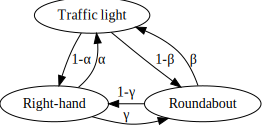
\includegraphics[width=13cm,height=13cm,keepaspectratio]{images/junctions}
\par\end{centering}
\caption{Conversion rates between junctions}
\end{figure}
\par\end{center}

The conversion will require the inputs to and from each type of intersection,
as these are not necessarily functions on each other. Some dependency
can be added later but that is independent of the current high-level
model. The required inputs are: $\alpha,\alpha\prime,\beta,\beta\prime$.
Each variable represents a conversion cost between two types of infrastructure.
The prime version of the variable is the reverse of the same building
procedure. The prime ($\prime$) will always reflect a destruction
e.g. demolishing an expensive piece of infrastructure and building
a cheaper one in place. The non-prime variable denotes the building
of a more expensive piece of infrastructure from a cheaper one.

By default conversions are defined between roundabouts and right-handed
intersections, traffic lights and right-handed intersections. Converting
a traffic light into a roundabout involves first removing the traffic
lights, essentially converting the junction into a right-handed intersection
and then rebuilding the right-handed intersection into a roundabout.
The same is true for converting a roundabout into a traffic light
intersection: first the roundabout must be converted into a right-handed
intersection and then traffic lights must be added to the intersection
thereby finishing the conversion into a traffic light intersection.
Therefore conversions between traffic lights and roundabouts are defined
as $\alpha+\beta$ and $\alpha\prime+\beta\prime$.

There are limiting factors to different types of junctions e.g. how
many roads it can intersect. The roundabout is famous for being able
to intersect five or more roads without any problem because of the
structure of it. Traffic lights can also have more roads than average
coming in and out of it. For the most part right-hand intersections
can handle at most four bidirectional roads. This is because human
attention cannot be focused to so many places at the same time. More
roads will translate to a more dangerous environment and will require
highly dedicated infrastructure. It is possible, but it's rarely seen
in the real world so it's not going to be considered in this research
as it reflects bad design principles. 

\subsection{Human factors}

Each training iteration the human factors get assessed according to
the city map. Human factors considered in the project are: 
\begin{enumerate}
\item How long roads are: roads too long get penalized. If the agent builds
a road to the furthest part of the city from a given junction the
face of the city will be too vastly modified. Each road longer than
half of the spread of the city will result in a penalty.
\item How many lanes a road is: each additional lane is more expensive to
build than the previous one. This is called expansion in construction
terms. If the agent builds an additional lane above a given threshold
a larger cost value will be accounted for.
\item Types of junctions: roundabouts are generally penalized and traffic
lights are rewarded. Roundabouts are good for vehicles as they provide
dynamic intersections but they don't provide possibilities for pedestrians
to cross. The traffic light intersection is the exact opposite: it
allows for pedestrians to cross while blocking high-speed motor traffic.
Right-hand intersections get no penalties. 
\end{enumerate}
The human factor aspect represents how livable a city is for a human.
This is a contradictory target with the motor vehicle aspect as motor
infrastructure and human infrastructure are mutually exclusive of each
other - the more motor vehicle infrastructure there is, the less human-centered
is the architecture.

\subsection{Motor vehicle aspect}

Each training iteration the simulation is ran for a given amount of
steps. 
\begin{enumerate}
\item Car distance and vehicles spawned: through the simulation it's measured
how much distance each car has taken and how long did they go. This
value is then added to the reward, so a higher value will result in
a larger reward. 
\item No nodes alone: if the graph is continuous the agent receives a reward
to learn to not leave out any junction from the traffic planning. 
\item Nodes alone: if there's a node that has no connection to any other
node, a penalty is added to the reward.
\end{enumerate}

\subsection{Other considerations}

The agent can take a number of actions and some are incorrect in a
given context. For this reason the agent's predicted Q-values are getting 
suppressed in these cases in order to make the agent avoid taking them:
\begin{enumerate}
\item Removing lane or road where there is currently nothing to remove (impossible).
\item Adding a lane or road where it has already reached maximum capacity
(defined by \emph{n\_lanes}).
\item Adding a lane or road with the starting and ending nodes being the
same (impossible).
\item Adding a junction where it is already built e.g. can't add a roundabout
where it's already a roundabout (impossible).
\end{enumerate}
This is an environmental restriction and is built into the framework
to help the agent with learning the rules.

\section{Network architecture}

The input for the neural network is the graph of the city represented
by an adjacency matrix. On each prediction pass the network has to
predict three values: \emph{end} and \emph{action} (in this order).
There were several implemented and tested architectures to achieve
reward maximization such as dense networks, ensemble networks, embedding
and graph convolutional networks. Below is the architectural description
of the architectures that measured the best in the testing environment
and served with enough insight so that comparison was worth it. 

The architecture has to predict ending node $B$ and action $a$ at
each iteration. The starting node is first given by the environment
at random, then each iteration the previous ending node will be assigned
as starting node. The naive implementation would be to use three separate
neural networks predict each of the variables. This method was experimented
on during training and the separate network architecture has been
measured to perform poorly. In fact the single-net architectures'
performance was so low that they didn't make it into the research
paper. However they can still be tried and experimented on in the
repository of the project. This architecture is erroneous in practice
as two complete neural networks would have to be trained separately.
The approach is redundant and can lead to information being lost and
increased computation times. 

In practice it's beneficial to make networks aware of each other's
predictions. This approach is reasonable as there are dependencies
between the variables: $A\Rightarrow B;\:A\Rightarrow a;\:B\Rightarrow a;\:x(A,B)\Rightarrow a$.
The ending node depends on the starting node, the action depends on
the starting starting node and ending node and the current state of
the infrastructure that is currently built between them. If these
dependencies are respected the true task can be learned better by
the neural network. 

The activation function used during the training was ReLu with an
optimizer of Adadelta and learning rate of 0.001. 

\pagebreak{}

\subsection{Graph convolutional architecture}

\subsubsection*{End prediction}

Below is the graph that is representative of the implemented deep
learning model responsible for predicting the ending node based on
structural information of the graph and the starting node that's given
in the current learning iteration. Each square node represents a deep
learning layer with trainable weights and each oval shaped node represents
some transformation in the neural network.

\begin{figure}[H]
\begin{centering}
\includegraphics[width=25cm,height=15cm,keepaspectratio]{images/gcnn_end}
\par\end{centering}
\caption{Graph convolutional network to predict the ending node}

\end{figure}

The input for the network is the adjacency matrix and the starting
node. First the adjacency matrix gets separated into node weights,
which is the state-definition matrix's main diagonal. The adjacency
matrix is the state-definition matrix with zeros on the main diagonal.
The graph convolutional layers take these variables as inputs and
produces an embedding for each node with a predefined size. The starting
node's embedding and features from the state-definition matrix is
selected using the starting node index. The embedding vector and the
feature vector are concatenated, flattened then passed to densely
connected layers. The output layer produces the state-action value
function which represents how good is it to select an ending node
from a given starting node. The agent will set the Q-values of the
ending nodes that have already been visited to $-\infty$.

\subsubsection*{Action prediction}

The second neural network is used to predict the action based on the
state, start and end. For this reason it's slightly more complex but
the general structure is the same as before. The two networks have
separably trainable weights and the same number of layers. The number
of neurons in the graph convolutional and fully connected layers can
be customized as preferred. During most of the experiments each of
the layers in the action prediction architecture had twice as many
neurons as the corresponding layer in the end prediction architecture.
The structure of the GCNN is as follows:

\begin{figure}[H]
\begin{centering}
\includegraphics[width=25cm,height=15cm,keepaspectratio]{images/gcnn_action}
\par\end{centering}
\caption{Graph convolutional network to predict the action}

\end{figure}

The inputs for the model are the state-definition matrix and the index
of the starting and ending nodes. Just as before the state matrix
gets separated into node weights and adjacency matrix in order to
bring them to a shape that's appropriate for the graph convolutional
layers. After the embeddings of the nodes have been extracted using
the convolutional operations the correct embedding features are selected
using the indices for start and end. The features of the start and
end are selected from the matrix using the same indices. The four
extracted vectors get concatenated into a single one that has the
shape of $2*embedding\_size+2*n\_nodes$ and the resulting 1-dimensional
vector gets passed to the fully connected layers. The amount of layers
at each neural pass can be customized though during training two hidden
layers were used. The output layer is used to predict the state-action
value function for the action which represents how lucrative is it
for the agent to be in a certain state and (given two nodes for the
start and end) take each action. The Q-values of the actions that cannot
be acted upon for each start, end pair get suppressed to $-\infty$. This
involves finding what the current junction is and how many lanes are
currently built between the starting and ending node. If for example
there are no lanes between the two junctions the agent cannot take
the remove\_lane action.

Some other considerations have also been taken into account while
designing the neural networks for the modeling process like regularization
through dropout which eliminates a node from the learning pass with
a predefined probability. This forces the agent to generalize better.
Another design aspect of the models is that before each training iteration
starts the model weights are initialized randomly using the Xavier
method also known as Glorot initialization \cite{glorot2010understanding}.
The resulting tensor will have weights uniformly sampled from $\mathcal{U}(-a,a)$
where 
\begin{equation}
a=gain\sqrt{\frac{6}{fan\_in+fan\_out}}
\end{equation}

Where gain is an optional scaling factor.

\subsection{Embedding architecture}

During running the experiments there were two other neural networks
with a very similar architectures that created the basis for comparison.
One that has used only embeddings (not graph convolutional) to make
predictions, and one that used only the graph features from the state
to determine the input for the dense connections. These models can
be understood as submodels of the GCNN architecture with slight modifications
so they are introduced briefly.

The embedding architecture uses embeddings used in natural language
processing to extract structural information from the graph. These
embeddings serve as low dimensional representations of the graph's
high dimensional and nonlinear structure. The embedding configuration
to predict the ending node is as follows:

\begin{figure}[H]
\begin{centering}
\includegraphics[width=8cm,height=8cm,keepaspectratio]{images/enn_end}
\includegraphics[width=8cm,height=8cm,keepaspectratio]{images/enn_action}
\par\end{centering}
\caption{Embedding network to predict the ending node (left) and the action
(right)}

\end{figure}

The input size for the densely connected layers is the same as the
embedding size in case of the ending node prediction network and twice
as much in the case of the action prediction network. Otherwise the
network works the same way as its graph convolutional counterpart.

\subsection{State-based architecture}

The last of the configurations is the most simple one. This is a naive
approach that served as an initial model and a baseline for comparison.
The state-based architecture doesn't employ embeddings or convolution.
It indexes into the state-definition matrix to acquire the features
specific to a node: to which other nodes and how many connections
it has and what type of intersection is currently set up in the junction
that it represents. The state-definition based architecture to predict
the starting and ending node: 

\begin{figure}[H]
\begin{centering}
\includegraphics[width=8cm,height=8cm,keepaspectratio]{images/snn_end}
\includegraphics[width=8cm,height=8cm,keepaspectratio]{images/snn_action}
\par\end{centering}
\caption{State-definition based architecture to predict the ending node (left)
and the action (right)}

\end{figure}

\newpage{}

\chapter{Results}

The following section will deal with introducing the findings of the
research. The machine learning task proved itself to be a very difficult
one even for modern machine learning methods. Several of the most
common approaches were implemented and tried in the environment however
only a few of them proved successful. There were several factors that
turned out to vastly influence the performance of the neural network
such as costs, environmental restrictions and hard coded rules. The
deep learning environment has more than 35 parameters, not counting
the ones needed to define and train the neural network. The main metric
that was used to measure the performance of the models was the cumulated
reward during each learning epoch. The comparison of networks in this
section includes networks trained with slightly different hyperparameters
but with the same rewarding scheme for a fair examination.

\section{The testing environment}

The main method for running the experiments was based on two notions: 
\begin{enumerate}
\item The agent should be able to reconfigure an already suboptimal environment
in order to make it more livable for humans while being able to provide
faster transportation for cars. This corresponds to the idea of planning
new expansions or destroying unnecessary roads in an already existing
environment.
\item The agent should be able to create a road configuration from only
the locations of the junctions, without having any roads or lanes
added in the first place. This mode becomes useful in the planning
phase of a green-field project where there's a need to connect predefined
places with the best possible cost effectiveness while providing fast
travel times in a motor vehicle. 
\end{enumerate}
For the above reasons two testing environments were created. They
are defined in such a way that there are multiple ways the agents
can reach a fast transportation time, but creating a humanly livable
environment at the same time remains a difficult task. The number and locations
of the nodes are exactly the same, the only difference is that there
are some connections added to one of the environments, the other one
remained empty. Out of the two distinct tasks the empty starting configuration 
can be classified as the harder one as the agent has no prior infrastructure to work
with. The images of the starting configurations can be seen below: 
\begin{enumerate}
\item The intersection that the agent will have to learn to optimize: 
\begin{figure}[H]
\begin{centering}
\includegraphics[width=8cm,height=8cm,keepaspectratio]{images/test_5_intersection}
\par\end{centering}
\caption{Predefined suboptimal environment: \emph{test\_5\_intersection}}
\end{figure}
\item The intersection that the agent will have to learn to build from scratch:
\begin{figure}[H]
\begin{centering}
\includegraphics[width=8cm,height=8cm,keepaspectratio]{images/test_5_intersection_empty}
\par\end{centering}
\caption{Predefined empty environment: \emph{test\_5\_intersection\_empty}}
\end{figure}
\end{enumerate}
By default all roads have one lane going in each direction, and all
junctions are configured to be right hand intersections. It's easy
to see that in the first image the configuration is suboptimal as
there are six roads meeting in one right-hand junction. This is erroneous
city design because of the danger of ambiguous right of way in the
interchange. Another key thing to note is that this intersection is
the bottleneck of the entire traffic system: by having six roads meet
at the same place all of the vehicles will have to wait for their
turn thereby likely causing a traffic jam. Traffic jams are measured
and penalized by the environment. 

Through the learning the agent is encouraged to either convert a right-hand
intersection to a traffic light intersection for safety, or to convert
it to a roundabout for speed. The traffic light intersection is more
expensive to build however it adds an extra layer of safety to the
configuration and for that it's rewarded. The more traffic light intersections
does an environment have the more it scores in the human livability
metric and the more roundabouts an environment has the more it scores
on the vehicular aspect of the evaluation phase. 

\section{Episodic rewards}

The following section will give an insight to the training rewards
for each main type of agent employed in the learning. They have the
same number of hidden layers, nodes, reward and environment configurations.
The goal here is to decide which agent can capture the nuances of
the traffic control problem better. The types of the agents are:
\begin{enumerate}
\item GCNN (Graph Convolutional Neural Network): a special architecture
that uses embeddings from graph convolutional layers as well as node
feature information indexed straight from the state-definition matrix. 
\item ENN (Embedding Neural Network): a configuration which uses solely node
embeddings as the input for the densely connected layers. The embeddings
here are the same as the ones used in natural language processing.
The input for the embeddings is the state-definition matrix. 
\item SNN: (State-based Neural Network): this one is the most naive configuration
that uses only the adjacency matrix representation of the state to
extract information on the nodes and connections of the graph. 
\end{enumerate}
During the training each agent was used to train for 1000 iterations
on both of the environments that were described earlier. A batch size
of 64 was used and the agents updated their weights after every 8
iterations. For the end prediction networks the dense layers' number
of neurons were {[}16,12,8{]} and for action prediction {[}32,16,8{]}.
The GCN layers had 10 hidden units as well as the dimensions of the
embeddings. As the agent will have to learn to optimize for long term
rewards a discount factor of 0.99 was used over the entire training procedure.
The strategy to optimize the rewards was epsilon greedy, where the
agent is taking random actions with a given probability which is large
at the beginning and decreases towards the end of the training. This
kind of approach incentivizes exploration at start and exploitation
in the end phase. Each training iteration the agent started out in
node 0, and had 15 occasions to take some action. The largest possible
reward was for adding a traffic light junction to one of the center
nodes or any of the agent-built intersections with enough inbound
roads. For each individual training the rewards of the agents were
logged for each step and each action. The training for training in
the suboptimal environment is the following: 

\begin{figure}[H]
\begin{centering}
\includegraphics[width=7cm,height=7cm,keepaspectratio]{images/scores_history_comparison_test_5_intersection}
\includegraphics[width=7cm,height=7cm,keepaspectratio]{images/windowed_scores_comparison_test_5_intersection}\includegraphics[width=7cm,height=7cm,keepaspectratio]{images/average_scores_comparison_test_5_intersection}
\par\end{centering}
\caption{Training results in the \emph{test\_5\_intersection} environment unsmoothed
(top), smoothed with a 50 size window (bottom left) and total average
(bottom right)}
\end{figure}

On the top is the reward for each episode. The rewards start out very
noisy in the beginning but they stabilize around some point after
a couple hundred iterations. In the bottom left there's the same exact
data row smoothed with a window size of 50 and on the bottom right
the same where for each episode the mean score was calculated. The
mean reward $\overline{r}$ at time step $t$: $\overline{r}_{t}=\frac{r_{0}+r_{1}+...+r_{t}}{t+1}$. 

The worst performing model was the state-based architecture, where
the embedding based and the graph convolutional models performed fairly
well. The ENN model gained a lot of high scores during the late phase
of the training giving it an advantage over the graph convolutional
network. The largest negative scores could also be attributed to the
SNN model, which also failed to converge around some reward value
by the end of the 1000th iteration. 

The other aspect to consider is the task of creating roads without
any prior configuration given: the \emph{test\_5\_intersection\_empty}
environment. The neural network agents were used to train with the
same hyperparameters as before and the results were logged. The results
are presented below:

\begin{figure}[H]
\begin{centering}
\includegraphics[width=7cm,height=7cm,keepaspectratio]{images/scores_history_comparison_test_5_intersection_empty}
\includegraphics[width=7cm,height=7cm,keepaspectratio]{images/windowed_scores_comparison_test_5_intersection_empty}\includegraphics[width=7cm,height=7cm,keepaspectratio]{images/average_scores_comparison_test_5_intersection_empty}
\par\end{centering}
\caption{Training results in the \emph{test\_5\_intersection} environment}
\end{figure}

This time the learning curves are diverging instead of all of them showing a steadily
increasing pace. The best performing model was the GCNN architecture
which learned to increase rewards over time. The embedding based network
was measured to be very unstable with the reward fluctuating with large
amplitude with the reward slowly decreasing over time. 
Only the graph convolution based model learned how to increase
rewards in the more difficult environment. Despite being noisier in
terms of score deviation it still measured higher than the embedding
based network which has converged around a value that is still lower
in score than the bottom mark of the GCNN model. 

Another insight to note is that in this case it wasn't possible for
the agents to add a traffic light intersection as the agent couldn't
return to the same node enough times to hit the traffic light inbound limit.

\section{Rewards for nodes}

The next aspect of evaluation is how much reward each agent has received
for building infrastructure to a given graph node. If the agent decided
to take action $a$ between the starting and ending nodes such that
$A\overset{a}{\rightarrow}B$ the reward will be accredited to the
cumulated reward of node $B$ as this was the one that the agent has
chosen (the starting node is chosen by the environment at first then
the previous ending node becomes the starting node). This type of
metric can give an insight to which nodes are more important in terms
of infrastructure building and planning. This roughly translates to
the idea of the state-value function $V(s)$ known in reinforcement
learning which expresses how profitable is it for the agent to be
in a certain state. The node based reward was calculated for each
of the agents for both of the predefined environments. These results
are from the same runs as seen in the previous chapter.

First the node based rewards for the \emph{test\_5\_intersection}
environment is presented for the three agents:

\begin{figure}[H]
\begin{centering}
\includegraphics[width=14cm,height=14cm,keepaspectratio]{images/node_reward_plot_node_weights_plot_test_5_intersection}
\par\end{centering}
\caption{Cumulated reward for graph nodes in the \emph{test\_5\_intersection}
environment}
\end{figure}

On the above plot each dot represents a node in the graph with the
actual $(x,y)$ coordinates. The size of the node corresponds to how
much reward did actions directed towards that node receive during
the learning. This information is also displayed next to the point
in numeric form in the million scale. 

Both the GCNN and the ENN models found the nodes in the middle of
the other nodes to be more reward prone than the others on the outside.
From the scoring we know that this is a better strategy than that
of the feature based network. It's intriguing to notice that some
of the outer nodes have negative cumulative rewards for the GCNN and
ENN models. The reason for this is that these are very likely to induce
heavy infrastructure costs as the roads become longer. Even more so
if the road is built from a distant node from the other side of the
city. Another underlying factor is that the agent receives a large
negative reward if a node is left out of the graph without any incoming
or outgoing nodes. For the SNN the rewards are distributed more evenly
among the inner and outer nodes which leads to the conclusion that
the model didn't develop enough experience to distinguish the state-values
of the nodes from each other. A key observation here is that an instant reward
for an action doesn't necessarily get followed with an instant positive reward.
Some road systems can only work if there are more interconnecting junctions
that achieve a high reward only if taken together. E.g. there's no point in 
having a 4-lane road if it ends in a single one-way street. The traffic flow 
gets disrupted which cannot be attributed to the larger road. The expansion
only makes sense if the connected roads get expanded too otherwise traffic jams
will occur.

The following plot is the same type of metric in the \emph{test\_5\_intersection\_empty}
environment as seen in the plot below: 

\begin{figure}[H]
\begin{centering}
\includegraphics[width=14cm,height=14cm,keepaspectratio]{images/node_reward_plot_node_weights_plot_test_5_intersection_empty}
\par\end{centering}
\caption{Cumulated reward for graph nodes in the \emph{test\_5\_intersection}
environment}
\end{figure}

This time the distributions are very uneven. In this testing environment
the models had a more difficult job. Also it was more easy to gain
reward as the initial reward is a highly negative value. For the GCNN
model the most profitable node was the one on the very right which
was unexpected given the nature of the task. In hindsight we know
that this turned out to be a good strategy to optimize the rewards.
In the case of the embedding based network the distribution of rewards
is very similar to the one that was seen in the other environment
with the exception of the bottom right node bringing an unusually
high reward given the outer location. For the state-based architecture
the top left neighborhood of nodes yielded the highest reward. The
bottom left and bottom middle nodes have been one of the least important
ones in all the cases. This couldn't be attributed to them being far
from the starting point as other nodes that are similarly far or even
further have been able to receive an even higher amount of reward.
What this means is that these nodes are not important from the aspect
of traffic flow and human livability.

\section{Embeddings}

In this section the embeddings of the networks are visualized to compare
their features in an untrained and trained state for the models where
it is possible (GCNN, ENN). Embeddings capture structural information
in a graph with the incentive that similar structures and neighborhoods
should have similar embeddings. 

An embedding size of 10 was used across the entire training procedure
so the datasets are in a 10-dimensional space. To be able to visualize
them a PCA based T-SNE model was applied using the same parameters
across all the datasets containing the values of the embeddings. This
method projects down a higher dimensional dataset into a lower dimensional
space by aggregating axes into latent variables called components.
To be able to visualize the dataset the number of components was set to two. 
There are in total two models with two neural networks each and two distinct 
states where the embeddings were captured.
\begin{enumerate}
\item GCNN, end prediction network:
\begin{figure}[H]
\begin{centering}
\includegraphics[width=14cm,height=14cm,keepaspectratio]{images/embeddings_before_after_end_gcnn_2023-05-05_15-03}
\par\end{centering}
\caption{End embeddings for the GCNN model untrained (left) and trained (right)}
\end{figure}
\item GCNN, action prediction network: 
\begin{figure}[H]
\begin{centering}
\includegraphics[width=14cm,height=14cm,keepaspectratio]{images/embeddings_before_after_action_gcnn_2023-05-05_15-03}
\par\end{centering}
\caption{Action embeddings for the GCNN model untrained (left) and trained
(right)}
\end{figure}
\item ENN, end prediction neural network:
\begin{figure}[H]
\begin{centering}
\includegraphics[width=14cm,height=14cm,keepaspectratio]{images/embeddings_before_after_end_enn_2023-05-05_22-54}
\par\end{centering}
\caption{End embeddings for the ENN model untrained (left) and trained (right)}

\end{figure}
\item ENN, action prediction neural network:
\begin{figure}[H]
\begin{centering}
\includegraphics[width=14cm,height=14cm,keepaspectratio]{images/embeddings_before_after_action_enn_2023-05-05_22-54}
\par\end{centering}
\caption{Action embeddings for the ENN model untrained (left) and trained (right)}
\end{figure}
\end{enumerate}
It can be well noted that the neural networks seem to have some kind
of idea on the similarity of the nodes in the untrained images. This
is because the embedding layers' weights were initialized randomly
and to get the embeddings the graph's adjacency matrix was passed
as an input to the neural network. On these plots the closer the dots
are the more similar they are according to the embedding layers. In
the untrained images they are more spaced out and in their trained
counterparts they are more closely bounded together. This is because
the networks learned which nodes are similar to which other nodes
in terms of structure and relationships to other nodes. Of course
structure is always changing, so always the beginning configuration
of \emph{test\_5\_intersection} was passed to the embedding layers
to have an equal basis of comparison. 

It's worth observing that the graph convolutional model made a larger
change in the embeddings while training the weights. This leads to
the conclusion that it has learned to distinguish them better and
use the structural and connection information from the graph in a more profitable
manner. The fact that it has performed better in the harder task than
the embedding based network proves this idea.

\section{Examples}

The following part is about giving examples on well scoring and badly
designed cities. After the training process the agents were used to
design a city for 15 discrete time steps, which means they had 15
opportunities to build or destroy infrastructure. One rule of building
is that no new junction gets created when two roads cross so the
vehicles cannot change from one road to the other one in the intersection
(essentially the crossing functions as a bridge). This was a way to
simplify the learning task but can be the ground for the continuation
of the research. If there are more lanes going between two junctions
they show up as a single line in the simulation. The reason for this
is that this research was focused on graphs and this is the most straightforward
way to display a graph. Some examples with words of analysis are:
\begin{enumerate}
\item GCNN, test\_5\_\emph{intersection}: this was one of the highest scoring
cities of the entire training procedure. The agent has learned that
if it connects the outer nodes then the traffic can be diverted between
these nodes giving them a much larger vehicle score. It has also realized
that in the center of the city many roads meet so it has added
traffic light intersections to the central nodes thereby gaining a
large positive reward in the human aspect scoring as well. 
\begin{figure}[H]
\begin{centering}
\includegraphics[width=8cm,height=8cm,keepaspectratio]{images/city_agent_gcnn_2023-05-03_23-33_test_5_intersection}
\par\end{centering}
\caption{GCNN model, evaluation, \emph{test\_5\_intersection}}

\end{figure}
\item GCNN, \emph{test\_5\_intersection\_empty}: this is a fairly well designed
city for the harder task. The structure is again very similar to the
one seen above: the outer nodes are connected for traffic flow, however
the agent hasn't learned to add traffic light intersections to the
inner junctions. For this goal it has to be highly adaptive as it
only has 15 time steps to create a traffic light junction, and this
type of intersection costs a lot and has the strictest criteria of
them all. 
\begin{figure}[H]
\begin{centering}
\includegraphics[width=8cm,height=8cm,keepaspectratio]{images/city_agent_gcnn_2023-04-29_18-06_test_5_intersection_empty}
\par\end{centering}
\caption{GCNN model, evaluation, \emph{test\_5\_intersection\_empty}}
\end{figure}
\item ENN, \emph{test\_5\_intersection}: this is a purely traffic oriented
map that is mainly focused around motor vehicles. The agent figured
out that it gets a high reward if it makes way for high-speed traffic.
There's an even higher reward if it also counts in the human aspect,
however this was not the case in this experiment. The agent however
learned that it can add roundabouts to the most used intersections
thereby speeding up motor traffic even more. This takes a one time
infrastructure building cost however speeds up the traffic from there
on. 
\begin{figure}[H]
\begin{centering}
\includegraphics[width=8cm,height=8cm,keepaspectratio]{images/city_agent_enn_2023-05-04_10-53_test_5_intersection}
\par\end{centering}
\caption{ENN model, evaluation, \emph{test\_5\_intersection}}
\end{figure}
\item ENN, \emph{test\_5\_intersection\_empty}: as seen in the analysis
of episodic rewards the ENN model had a clearly subpar performance
on this testing environment. This can be noted in the organization
of the map below as well: there are no special types of intersections,
the graph isn't continuous and there are clearly entry points between
which traveling includes needlessly long detours. This city scored
very low during the testing and our human instincts support this evidence.
This is not a city that anyone in their sane mind would design or
live in.
\begin{figure}[H]
\begin{centering}
\includegraphics[width=8cm,height=8cm,keepaspectratio]{images/city_agent_enn_2023-05-04_22-59_test_5_intersection_empty}
\par\end{centering}
\caption{ENN model, evaluation, \emph{test\_5\_intersection\_empty}}
\end{figure}
\item SNN, \emph{test\_5\_intersection}: this is a fairly well-designed
city at first glance, however the agent has missed out on a lot of
opportunities to gain a large reward so the others have outperformed
it. It has added a lot of roundabouts to almost all the outer nodes
which resulted in two things: a negative score as per the cost of
building the infrastructure while not being able to significantly
speed up traffic as these intersections have at most three inbound
roads but most often one or two. What the agent did right however
is that it has added a roundabout to the intersection with the most
inbound lanes in order to speed up traffic flow and a traffic light
to the other central junction so that it gets the bonus for the human
element of the scoring process. Despite the agent having the right
idea, it has failed to produce good results on the long term.
\begin{figure}[H]
\begin{centering}
\includegraphics[width=8cm,height=8cm,keepaspectratio]{images/city_agent_snn_2023-05-04_14-28_test_5_intersection}
\par\end{centering}
\caption{SNN model, evaluation, \emph{test\_5\_intersection}}
\end{figure}
\item SNN, \emph{test\_5\_intersection\_empty}: one of the worst models
in the history of the project was made on this test run. The agent
had a steadily decreasing score during the training. It has failed
to realize that adding roads will increase traffic speeds and connecting
them in a way that they are reachable from one another will yield
an even higher reward. It has failed to realize that adding roundabouts
only makes sense if there are multiple inbound roads to the intersection
so it has added three roundabouts with only two incoming lanes. The
discontinuity of the graph and the fact that some nodes remained without
any connections to others also yielded a large negative reward.
This is clearly a wrong configuration and is shown as an example to
demonstrate the difference between an agent of superior and inferior
performance in the testing environments. 
\begin{figure}[H]
\begin{centering}
\includegraphics[width=8cm,height=8cm,keepaspectratio]{images/city_agent_snn_2023-05-04_20-30_test_5_intersection_empty}
\par\end{centering}
\caption{SNN model, evaluation, \emph{test\_5\_intersection\_empty}}
\end{figure}
\end{enumerate}
\newpage{}

\chapter{Conclusion}

The task of traffic control using reinforcement learning has proved
itself to be very difficult in terms of modeling, optimization and
simulation. The need for a realistic simulation environment is large,
however with such a simulation environment comes a large number
of variables which need to be handled by the machine learning model.
It's a very time consuming problem to find the rewarding scheme that
reflects what a human expects from a well-designed city while being
able to combine it with the capability of a neural network to uncover
insights from factors underlying the data. For this reason an insight is that 
very thorough research should precede the modeling phase where the cost of
each infrastructure building and destroying is determined specifically to 
the area and economical setting where the project is being executed. 
With the gained experience and understanding the following paragraphs 
will deal with answering the research hypotheses supposed in the beginning of the study. 

\section*{Hypotheses}
\begin{enumerate}
\item Can traffic flow and driver behavior be modeled inside a reinforcement
learning environment accurately enough for it to be representative
of the real world?
\begin{description}
\item [{-}] The bottleneck of the learning process is running the simulation
after each action of the reinforcement learning agent. With the fairly
simple simulation environment training times could take up to 24 hours
to finish 1000 episodes. Even so sometimes the agents were measured
to be underfit, showing a need for more actions inside one episode
and for more episodes inside the training. To create an environment
that accurately represents the real world and to play with it inside
the environment would take heavy tolls on the time and budget of the
laboratory, however technologically it is possible. The environment
employed in this research wasn't nearly as complicated as the real
world, however it was enough for the agent to learn the main city
design guidelines that it was designed to do. It's also worth pointing out 
that so far these models didn't perform nearly as well as a professional would. 
The hypothesis is supported. 
\end{description}
\item Can predefined road configurations be optimized for traffic flow,
human livability and cost efficiency at the same time? 
\begin{description}
\item [{-}] It was shown in the research that if passed a configuration
with infrastructure already present, the agent will learn to take
the already existing structure and start building on top of it while
using its advantages e.g. connecting the outer nodes in order to eliminate
the middle intersections as the bottleneck of the process. Human livability
factors were also learned through adding traffic light intersections
and respecting the cost of adding new lanes or additional lanes next
to existing ones. With the right reward configuration the human livability
will be respected as much as needed for the current setup. The hypothesis
is validated.
\end{description}
\item Is there a single neural network architecture that can achieve the
optimization in every configuration or there is a need for a more
complex neural network as the complexity of the graph increases? 
\begin{description}
\item [{-}] There were experiments that were ran using a single, three
headed neural network model. It didn't make it to the documentation
because it was performing worse than random guessing. However it can
still be downloaded in the repository of this project. The single
network architectures didn't learn anything other than repeating the
same exact action when prompted. One key advancement was separating
the neural network into two distinct ones: one that predicts the ending
node and another one that predicts the action. Random weight initialization
and dropout have also helped dealing with their proneness to overfitting.
Another key function was restricting the actions of the model to render
invalid when a given action was not possible. All these evidences
show that such a model has a lot of rules to learn and things such
as exploration and restriction of actions helps it make the right
decisions and improve the reward on the long run. The hypothesis is
rejected.
\end{description}
\end{enumerate}

\section*{Lastly}

The purpose of this research was to develop a reinforcement learning
model that can optimize traffic flow in a city by building roads,
lanes and intersections between predefined nodes that are defined
on a user friendly interface. The model takes into account how
fast and dynamically does traffic flow and how welcoming a city is
to its residents: the number of lanes and infrastructure cost have
to be minimal while also minimizing the time taken to travel between
junctions. To conduct the experiment, the machine learning model uses
a simulated environment that incorporates an intelligent driver model
in order to provide the most accurate mapping between real life and
the modeled environment. The simulator proved itself to be sufficient
for the small scale experiment however if the project is to be used
in the industry there's a large need for an environment that can handle
large amounts of data with a heavy graphics load.

Use cases of the research include optimizing current road structure
and generating new paths between already existing cities or settlements
that use the least amount of taxpayer money while also providing them
with the fastest travel times. The developed framework can also be
generalized for uses in public transport: using smart forecasting
to optimize bus or train lanes to cover the most area, for as many
people as possible. A future extension may include smart setting of
traffic signal cycles to better divert traffic. Different types of
vehicles and different driver behaviors would also help make the simulation
environment more realistic in the sense that traffic flow would behave
even more like in real life. It's also worth noting that this would
add even more noise to an already very noisy system. One key thing
that could prove itself useful is factoring in the type of terrain
that the roads are built on and being able to assign different infrastructure
costs to different areas of land.

The most important insight was how different reinforcement learning
algorithms can be made robust enough to handle a task with a lot of
noise and variation. The methodology of creating such models is well
known however this problem required a combination of regularization
and restriction that is very task specific. The application of these
methods was measured to yield results that serve with understanding
that can be used in real-world projects as well. The application of
this technology itself is very new with graph convolutional neural
networks being only a few years old at the time of releasing this
research. I sincerely hope that my research will serve with the advancement
of traffic control technologies for both the benefit of humans and
motor vehicles.

\newpage{}

\printbibliography

\listoffigures

\listoftables

\end{document}
